% !TeX spellcheck = en_US

\chapter{Generating minimal DFAs} \label{ch:2}

We seek algorithms for generation of minimal DFAs that fulfilling the conditions defined in the requirements analysis section~\ref{ch:1:determined-requirements}. We formally subsume these conditions via the GenerateNewMinimalDFA-problem:
\begin{definition}[GenerateNewMinimalDFA] $ $ \\
	$ $ \vspace{-0.4cm} \\
	\noindent $\underline{\emph{Given:}}$
	\vspace{-0.5cm}
	\begin{align*}
	\mathcal{Q}_{sol} \in \mathbb{N}\ \ \ & \emph{number of states} \\
	a \in \mathbb{N}\ \ \ & \emph{alphabet size} \\
	f \in \mathbb{N}\ \ \ & \emph{number of final states} \\
	m_{min}, m_{max} \in \mathbb{N}\ \ \ & \emph{lower and upper bound for $\mmD$-value} \\
	p \in \{0,1\}\ \ \ & \emph{planarity-bit}
	\end{align*}
	\noindent $\underline{\emph{Task:}}$ \emph{Compute, if it exists, a solution DFA $A_{sol}$ with}
	\begin{itemize}
		\item $|Q_{sol}|=\mathcal{Q}_{sol}$, $|\Sigma_{sol}|=a$, $|F_{sol}|=f$
		\item $m_{min} \le \mmD(A_{sol}) \le m_{max}$
		\item $A_{sol}$ \emph{being planar iff} $p = 1$
		\item $A_{sol}$ \emph{being new}
	\end{itemize}
\end{definition}
\noindent We consider different approaches to solve this problem, of which those using trial-and-error will be discussed most broadly.

Note that the presented algorithms will not be able to compute all of $\mathfrak{A}_{min}$ since we are going to exclude minimal DFAs that are practical isomorph to already found ones.

\section{Using trial and error}

We will develop an algorithm that makes partly use of the trial-and-error paradigm to find matching DFAs. The approach here is as follows:

Firstly a \emph{test} DFA $A_{test}$ is generated by use of either randomness or enumeration. Alphabet size and number of (final) states will already be correct. On this DFA then tests will be executed, to check if it is minimal, planar (if wished) and new. If this is the case, $A_{test}$ will be returned, if not, new test DFAs are generated until all tests pass.

By constructing test DFAs with already correct alphabet size and number of (final) states we are able to subdivide the search space of DFAs in advance into much smaller pieces which are in particular finite.

\gregor{How much smaller? Why now finite?}

\vspace{0.2cm}
\begin{algorithmic}[1]
	\Function{BuildNewMinimalDFA-1\ }{$\mathcal{Q}_{sol}, a, f, m_{min}, m_{max} \in \mathbb{N}, p \in \{0,1\}$}
		\While {True}
		
			\vspace{0.2cm}
		
			\State generate DFA $A_{test}$ with $|Q|, |\Sigma|, |F|$ matching $\mathcal{Q}_{sol}, a, f$
			
			\vspace{0.2cm}
			
			\If {$A_{test}$ not minimal \textbf{or not} $m_{min} \leq \mmD(A_{test}) \leq m_{max}$}
				\State \textbf{continue}
			\EndIf
			
			\If {$p = 1$ \textbf{and} $A_{test}$ is not planar}
				\State \textbf{continue}
			\EndIf
			
			\If {$A_{test}$ is not new}
				\State \textbf{continue}
			\EndIf
			
			\vspace{0.2cm}
			
			\State\Return $A_{test}$
		\EndWhile
	\EndFunction
\end{algorithmic}
\vspace{0.2cm}
We will complete this algorithm by resolving how the tests in lines $4, 6$ and $8$ work and by showing two methods for generation of automatons with given restrictions of $|Q|, |\Sigma|$ and $|F|$.

\subsection{Ensuring $A_{test}$ is minimal and $\mmD(A_{test})$ is correct}

In order to test, whether $A_{test}$ is minimal, we could simply use the minimization algorithm and compare the resulting DFA and $A_{test}$ using an isomorphy test. However it is sufficient to ensure, that no equivalent or unreachable states exist.
\gregor{minimality planarity complete under isomorphy}

To get $\mmD(A_{test})$, we have to run \CompDist\ entirely anyway. Hence we can combine the test for equivalent states with computing the DFAs $\mmD$-value:
\vspace{0.2cm}
\begin{algorithmic}[1]
	\Function{HasEquivalentStates}{$A$}
		\State $depth \gets 0$
		\State $M \gets \{ (p,q), (q,p)\ |\ p \in F, q \notin F \}$
		\Do
			\State $depth \gets depth + 1$
			\State $M' \gets \{ (p,q)\ |\ (p,q) \notin M \land \exists \sigma \in \Sigma \colon (\delta(p,\sigma), \delta(q,\sigma)) \in M \}$
			\State $M \gets M \cup M'$
		\doWhile {$M' \neq \emptyset$}
		\State $hasDupl \gets | \{ (p,q)\ |\ p \neq q \land (p,q) \notin M \} | > 0$
		\State \Return $hasDupl, depth$
	\EndFunction
\end{algorithmic}
\vspace{0.2cm}
Since \CompDist\ basically computes all distinguishable state pairs $\not\sim_A$, we test in line $9$, whether there is a pair of distinguishable states not in $\not\sim_A$.

Regarding the unreachable states, we can just use \CompUnr\ and test whether the computed set is empty:
\vspace{0.2cm}
\begin{algorithmic}[1]
	\Function{HasUnreachableStates}{$A$}
	\State \Return $|\CompUnr(A)| > 0$
	\EndFunction
\end{algorithmic}

\subsection{Ensuring $A_{test}$ is planar}

There exist several algorithms for planarity testing of graphs. In this work, the library \emph{pygraph}\footnote{\url{https://github.com/jciskey/pygraph}} has been used, which implements the Hopcroft-Tarjan planarity algorithm. More information on this can be found for example in this~\cite{Koc93} introduction from William Kocay. The original paper describing the algorithm is~\cite{HT74}.

\subsection{Ensuring $A_{test}$ is new}

In our requirements we stated, that we wanted the generated solution DFA to be new, meaning not practically isomorph to any previously generated solution DFA. This implies the need of a database, that allows saving and loading DFAs. We name this database \emph{DB1}. Assuming the database is relational, the following scheme is proposed:
\begin{center}
	\begin{tabular}{c c c c c c}
	$|Q_A|$ & |$\Sigma_A$| & $|F_A|$ & $\mmD(A)$ & $isPlanar(A)$ & $encode(A)$
	\end{tabular}
\end{center}
With this scheme we can fetch once all DFAs matching the search parameters. Thus we need not fetch all previously found DFAs every time, but only those that are relevant. Afterwards we must only check whether any practical isomorphy test on the current test DFA and one of the fetched DFAs is positive. If any test DFA passes all tests and is going to be returned, then we have to save that DFA in the database.

A more concrete specification of this proceeding is shown below, embedded in the main algorithm:
\vspace{0.2cm}
\begin{algorithmic}[1]
	\Function{BuildNewMinimalDFA-2\ }{$\mathcal{Q}_{sol}, a, f, m_{min}, m_{max}, p$}
	
		\vspace{0.2cm}
	
		\State $l \gets$ all DFAs in DB1 matching $\mathcal{Q}_{sol}, a, f, m_{min}, m_{max}, p$
		
		\vspace{0.2cm}
		
		\While {True}
		
		\vspace{0.2cm}
		
			\State $\ldots$
			\If {$A_{test}$ is practical isomorph to any DFA in $l$}
				\State \textbf{continue}
			\EndIf
			
			\vspace{0.2cm}
			
			\State save $A_{test}$ and its respective properties in DB1
			\State\Return $A_{test}$
		\EndWhile
	\EndFunction
\end{algorithmic}
\vspace{0.2cm}

\subsection{Option 1: Generating $A_{test}$ via Randomness}

We now approach the task of generating a random DFA whereas alphabet and number of (final) states are set.

Corollary~\ref{ch:1:cor:all-min-dfa-ism} tells us, that the states names are irrelevant for the minimality of a DFA, therefore we will give our generated DFAs simply the states $e_1, \ldots, e_{\mathcal{Q}_{sol}}$. For alphabet symbols this is not given. But since we \gregor{TODO minimality and planarity complete under isomorphy}

We can state, that our start state is $e_1 \in Q$, since we can apply an isomorphism to every DFA, such that its start state is renamed to $e_1$.

The remaining elements that need to be defined are $\delta$ and $F$. The set of final states is supposed to have a size of $f$ and be a subset of $Q$. Therefore we can simply choose randomly $f$ distinct states from $Q$.

The transition function has to make the DFA complete, so we have to choose an ``end'' state for every combination in $Q \times \Sigma$. There is no restriction as to what this end state shall be, so given $e \in Q$ and $\sigma \in \Sigma$ we can randomly choose an end state from $Q$.

With defining how to compute $\delta$ we have covered all elements of a DFA.

\vspace{0.2cm}
\begin{algorithmic}[1]
	\Function{BuildNewMinimalDFA-3a\ }{$\mathcal{Q}_{sol}, a, f, m_{min}, m_{max}, p$}
	
		\vspace{0.2cm}
	
		\State $l \gets$ all DFAs in DB1 matching $\mathcal{Q}_{sol}, a, f, m_{min}, m_{max}, p$
		\State $Q \gets \{e_1, \ldots, e_{\mathcal{Q}_{sol}}\}$
		\State $\Sigma \gets \{\sigma_1, \ldots, \sigma_a\}$
		
		\vspace{0.2cm}
		
		\While {True}
		
		\vspace{0.2cm}
		
			\State $\delta \gets \emptyset$
			\For {$e$ \textbf{in} $Q$}
				\For {$\sigma$ \textbf{in} $\Sigma$}
					\State $e' \gets$ random chosen state from $Q$
					\State $\delta \gets \delta \cup \{((e,\sigma),e')\}$
				\EndFor
			\EndFor
			\State $s \gets e_1$
			\State $F \gets$ random sample of $f$ states from $Q$
			\State $A_{test} \gets (Q, \Sigma, \delta, s, F)$
			
			\vspace{0.2cm}
			
			\If {$A_{test}$ not minimal \textbf{or not} $m_{min} \leq \mmD(A_{test}) \leq m_{max}$}
			\State \textbf{continue}
			\EndIf
			
			\If {$p = 1$ \textbf{and} $A_{test}$ is not planar}
			\State \textbf{continue}
			\EndIf
			
			\If {$A_{test}$ is isomorph to any DFA in $l$}
			\State \textbf{continue}
			\EndIf
			
			\vspace{0.2cm}
			
			\State save $A_{test}$ and its respective properties in DB1
			\State\Return $A_{test}$
		\EndWhile
	\EndFunction
\end{algorithmic}
\vspace{0.2cm}

\subsection{Option 2: Generating $A_{test}$ via Enumeration}

% enumerating instead of random

The second method of test DFA generation is based on the idea, that instead of randomly generating $F$ and $\delta$, we could just enumerate through all possible final state sets and transition functions.

% finite enumerations, how many

Both enumerations are finite, given $\mathcal{Q}_{sol}$ and $a$. Having a requirement of $f$ final states, then $\mathcal{Q}_{sol}$ choose $f$ is the number of possible $F$-configurations. On the other hand there are ${\mathcal{Q}_{sol}}^{\mathcal{Q}_{sol}*a}$ possible $\delta$-configurations: We have to choose one of $\mathcal{Q}_{sol}$ possible end states for every combination in $Q\times\Sigma$ - so $\mathcal{Q}_{sol}*a$ times.

% Two fields

Again we will call our states and symbols w.l.o.g.\ $e_1,\ldots,e_{\mathcal{Q}_{sol}}$ resp.\ $\sigma_1,\ldots,\sigma_a$. We will represent the state of an enumeration with two fields $F_F$ and $F_\delta$. The first field shall have $\mathcal{Q}_{sol}$ Bits, whereas Bit $F_F[i] \in [0,1]$ represents the information, whether $e_i$ is a final state or not. The second field shall have $\mathcal{Q}_{sol}*a$ entries containing state indices, such that entry $F_\delta[i * a + j] = k, k\in[1,\mathcal{Q}_{sol}]$ says, that $\delta(e_i, \sigma_j) = e_k$. These semantics are illustrated in figure~\ref{fig:dfa_enum_bit_fields}.

% -- EX example of the two fields and their meaning

\begin{figure}
	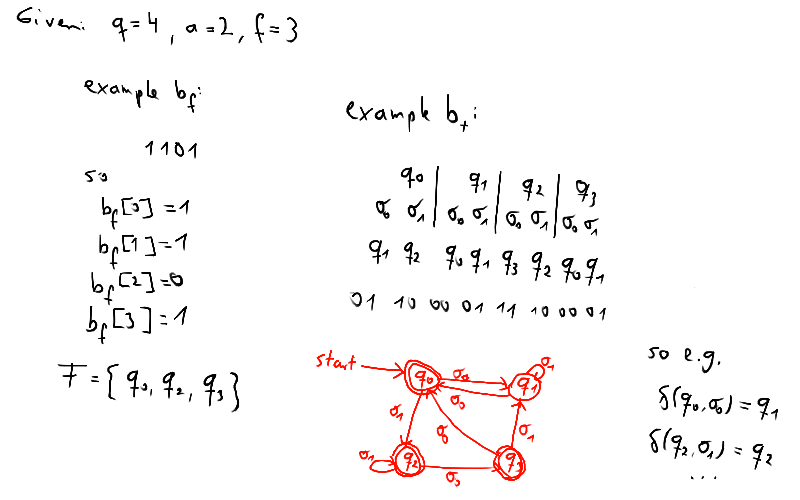
\includegraphics[width=\linewidth]{images/dfa_enum_bit_fields.png}
	\caption{Example for two possible configurations of the fields $F_F$ and $F_\delta$ given $\mathcal{Q}_{sol}, a$ and $f$. Below the corresponding DFA is drawn.}
	\label{fig:dfa_enum_bit_fields}
\end{figure}

% how to compute next DFA

Given an enumeration state $b_f, b_t$ and $\mathcal{Q}_{sol}, a, f$ we will then compute the next DFA based on this state as follows. We will treat both fields as numbers, $F_f$ as binary and $F_\delta$ as $\mathcal{Q}_{sol}$-ary. To get to the next DFA, we will first increment $F_\delta$ by $1$. If $F_\delta = 1 \ldots 1$, then we increment $F_F$ until it contains $f$ ones (again) and set $F_\delta$ to $0 \ldots 0$. This behavior is summarized in the following algorithm: \gregor{Clarify what happens at 11111...}
\vspace{0.2cm}
\begin{algorithmic}[1]
	\Function{IncrementEnumProgress\ }{$F_F, F_\delta, \mathcal{Q}_{sol}, a, f$}
	\State add $1$ to $(F_\delta)_{\mathcal{Q}_{sol}}$
	\If {$F_\delta = 0 \ldots 0$}
		\While {$\#_1(F_F) \neq f$} \Comment{if the number of 1s in $F_F$ is not $f$}
			\State add $1$ to $(F_F)_2$
			\If {$F_F = 0\ldots 0$}
				\State \Return $\bot$
			\EndIf
		\State $F_\delta = 0 \ldots 0$
		\EndWhile
	\EndIf
	\State \Return $F_F, F_\delta$
	\EndFunction
\end{algorithmic}
\vspace{0.2cm}
The example in figure~\ref{fig:dfa_enum_incr} illustrates such increments.

% EX -- example of an enumProgress increment

\begin{figure}
	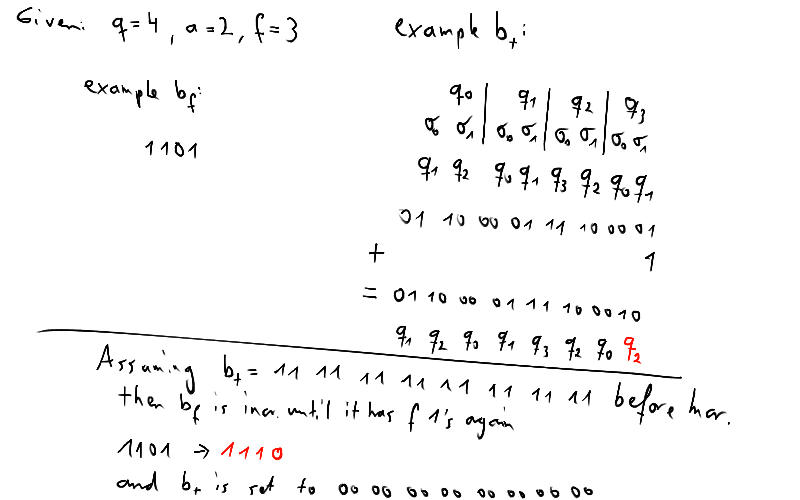
\includegraphics[width=\linewidth]{images/dfa_enum_incr.png}
	\caption{The upper half shows how a $F_\delta$-increment results in a change in the resulting DFAs transition function: $\delta(e_3, \sigma_1) = e_1$ becomes $\delta(e_3, \sigma_1) = e_2$. The lower half shows what happens, if $F_\delta$ has reached its end.}
	\label{fig:dfa_enum_incr}
\end{figure}

Based on the incremented bit-fields the new DFA can be build according to the semantics defined above:
\vspace{0.2cm}
\begin{algorithmic}[1]
	\Function{DFAfromEnumProgress\ }{$F_F, F_\delta, \mathcal{Q}_{sol}, a, f$}
	\State $Q \gets \{e_1, \ldots, e_{\mathcal{Q}_{sol}}\}$
	\State $\Sigma \gets \{\sigma_1, \ldots, \sigma_a\}$
	\State $\delta \gets \emptyset$
	\For {$i$ \textbf{in} $[1, \ldots, \mathcal{Q}_{sol}]$}
		\For {$j$ \textbf{in} $[1, \ldots, a]$}
            \State $\delta(e_i, \sigma_j) = e_{F_\delta[i * a + j]}$
		\EndFor
	\EndFor
	\State $s \gets e_1$
	\State $F \gets \{\ e_i\ |\ i \in [1, \ldots, \mathcal{Q}_{sol}] \land F_F[i] = 1\ \}$
	\State \Return $(Q, \Sigma, \delta, s, F)$
	\EndFunction
\end{algorithmic}
\vspace{0.2cm}
The initial field values are each time $0\ldots 0$. Note how construction and use of these fields results in DFAs with correct alphabet size and number of (final) states. An enumeration can finish either because a matching DFA has been found or all DFAs have been enumerated.

% saving enumProgress for later progression

Once the enumeration within a call of \textsc{BuildNewMinimalDFA} has been finished, it is reasonable to \emph{save} the enumeration progress (meaning the current content of $F_F, F_\delta$), such that during the next call enumeration can be resumed from that point on. The alternative would mean, that the enumeration is run in its entirety until that point again, whereas all so far found DFAs would be found to be not new. Thus we introduce a second database $DB2$ with the following table:
\begin{center}
	\begin{tabular}{c c c c c c}
		$|Q_A|$ & |$\Sigma_A$| & $F_F$ & $F_\delta$
	\end{tabular}
\end{center}
We reduce the enumeration room for each calculation.
\vspace{0.2cm}
\begin{algorithmic}[1]
	\Function{BuildNewMinimalDFA-3b\ }{$\mathcal{Q}_{sol}, a, f, m_{min}, m_{max}, p$}
	
		\vspace{0.2cm}
	
		\State $l \gets$ all DFAs in DB1 matching $\mathcal{Q}_{sol}, a, f, m_{min}, m_{max}, p$
		\State $F_F, F_\delta \gets$ load enumeration progress for $\mathcal{Q}_{sol}, a, f, p$ from DB2
		
		\vspace{0.2cm}
		
		\While {True}
		
			\vspace{0.2cm}
		
			\If {$F_F, F_\delta$ is finished}
				\State save $F_F, F_\delta$
				\State\Return $\bot$
			\EndIf
			\State $A_{test} \gets$ next DFA based on $F_F, F_\delta$
			
			\vspace{0.2cm}
			
			\If {$A_{test}$ not minimal \textbf{or not} $m_{min} \leq \mmD(A_{test}) \leq m_{max}$}
				\State \textbf{continue}
			\EndIf
			
			\If {$p = 1$ \textbf{and} $A_{test}$ is not planar}
				\State \textbf{continue}
			\EndIf
			
			\If {$A_{test}$ is isomorph to any DFA in $l$}
				\State \textbf{continue}
			\EndIf
			
			\vspace{0.2cm}
			
			\State save $F_F, F_\delta$ in DB2
			\State save $A_{test}$ and its respective properties in DB1
			\State\Return $A_{test}$
		\EndWhile
	\EndFunction
\end{algorithmic}
\vspace{0.2cm}

\section{Alternative approach: Building $m(i)$ bottom up}

Build $m$ from $m$-\CompDist\ iteratively. (Why would this basically result in running \CompDist\ all the time?)

\section{Related Research}

Nicaud provides an overview of results on random generation and combinatorial properties of DFAs in ~\cite{Nic14}. We will outline relevant related research.

\subsection{DFA generation}

Nicaud's summary indicates, that research has focused on randomized generation of accessible, but not minimal DFAs so far. In the following we will sketch some approaches that have come up.

\paragraph*{Using the recursive method.}

Champarnaud and Paranthoën~\cite{CP05} continue ideas started by Nicaud in his thesis~\cite{Nic00}. Let $\mathfrak{F_{n,m}}$ be the set of extended $m$-ary trees of order $n$. These trees are characterized by a partitioning $V = N \uplus L$ with $|N| = n$ and $v \in N \Rightarrow d^+(v) = m$ and $v \in L \Rightarrow d^+(v) = 0$. We define the following set of tuples using $s=n(m-1)$:
\[
    \mathfrak{R_{m,n}} = \{\ (k_1,\ldots,k_s) \in \mathbb{N}^s\ |\ \forall i\in [2,s]\colon k_i \geq \left\lceil\frac{i}{m-1}\right\rceil\ and\ k_i \geq k_{i-1}\ \}
\]
In~\cite[p. 6]{CP05} it is shown that there exists a bijection $\varphi$ between $\mathfrak{F_{n,m}}$ and $\mathfrak{R_{m,n}}$ which maps to $k_i$, $i\in[1,s]$ of a tuple the number of leaves visited before the $i$th leaf in a tree. The connection to accessible DFAs is established by proving that  ``transition structures\footnotemark''\ with $|Q|=n$, $|\Sigma|=m$ reduced to the set of the smallest paths from the $s$ to each other state are in bijection with extended $m$-ary trees of order $n$ (see~\cite[p. 8]{CP05}).

As a consequence they are able to construct a random generation of accessible complete DFAs using the ``recursive method'' from~\cite{NW78} which generates $n$-tuples~\cite[p. 10]{CP05}. Nicaud states in his survey that the algorithm's runtime is $\mathcal{O}(n^2)$ but notes, that generation of DFAs with more than ``a few thousand states'' is practically hard to do~\cite[pp. 10-11]{Nic14}.
\footnotetext{Those are essentially DFAs without final state sets.}

Almeida et.\ al.~\cite{AAA09, AMR09, RMA05} present and implement methods using a string-encoding of DFAs for exact enumeration and random generation of DFAs. Nicaud~\cite[p. 11]{Nic14} states in a remark, that this approach uses the same recursive method and differs only in the DFA encoding.

\paragraph*{Using Boltzmann sampler.}

Bassino, David and Nicaud present and implement a more efficient random generator of accessible complete DFAs in~\cite{BDN07, BN07}. Their idea is based on so called Boltzmann samplers. This framework of samplers is characterized in particular by the fact that the size of its generated objects are not fixed but in an interval around a given input size - this stands in opposition to most random generators in literature~\cite[p. 2]{DFL04}.

In~\cite{BN07} the authors use a Boltzmann sampler to generate set partitions that are shown to be in bijection with so called box diagrams~\cite[p. 8]{BN07} which are in turn in bijection to accessible complete DFAs~\cite[p. 4]{BN07}. They thus acquire an average runtime complexity of $\mathcal{O}(n^{3/2})$ for a single random generation.

\paragraph*{Using a rejection algorithm.}

Carayol and Nicaud~\cite{CN12} give a simple algorithm with the same runtime complexity. They use a result stating that the size of accessible DFAs is concentrated around some computable value. In the end random possibly inaccessible DFAs of a specific size are generated, of which afterwards all unreachable states are deleted. This is thus essentially a rejection algorithm with clever generation of test DFAs. They furthermore show that allowing approximate sampling with the number of states being in $[n-\varepsilon\sqrt{n}, n+\varepsilon\sqrt{n}]$ results in linear expected runtime.

\paragraph*{Others and comparison to algorithm presented in this work.}

In his survey Nicaud mentions a paper by Bassino and Sportiello~\cite{BS13} that yields random generation of accessible DFAs in expected linear time. This work will not be discussed further here.

In this work we use a rejection algorithm that generates test DFAs either by randomization or by enumeration. Both methods implement a naive approach. The generated test DFAs are not necessary minimal and in particular not necessary accessible as in~\cite{CN12}. The enumeration method uses encodings of DFAs similar to those used by Almeida et.\ al.~\cite{RMA05}.

\subsection{Combinatorial properties of DFAs}

Concerning combinatorial properties of DFAs, several authors (e.g.~\cite{BN07, DKS02, HJ14}) consider a work from Vyssotsky~\cite{Vys59} in the Bell laboratories to be the first on this subject. A contribution by Korshunov~\cite{Kor78} is often cited in this regard, for he firstly ``determines an asymptotic estimate of the number of accessible complete and deterministic $n$-state automata over a finite alphabet''~\cite{BDS11}.

\begin{itemize}
	
	% Combinatorial
	
    \item 2002 \cite{DKS02} Number of distinct $n$-$k$ minimal DFAs except isomorphy. Asymptotic estimates and explicit numbers.
    
    \item 2011 \cite{BDS11} Determined the fraction of minimal automata among accessible complete DFAs.
    
    \item 2013 \cite{BK13} Number of essential states for random $n$-$k$-DFAs is $\alpha_k n + \mathcal{O}(\sqrt{n}\log n)$ for a constant $\alpha_k$.
    
    % Empirical
    
   	\item  In their experimental evaluation\cite[p. 14]{CP05} Champarnaud and Paranthoën notice a empirical probability of $0.8$, that a generated DFA is minimal.
   	
   	\item Empirical table on min.\ DFAs for many state and alphabet sizes \cite[p. 11]{AMR09}. Diagram for rate of min.\ DFAs for two given $k,n$. Confirms empirical probability by CP.
   	
   	\item 2007 \cite{BDN07} Empirical on min.\ DFAs per state size, redundant states per state size.
\end{itemize}
\gregor{TODO}

%\begin{itemize}
%    \item 2002 \cite{DKS02} Number of distinct $n$-$k$ minimal DFAs except isomorphy. Asymptotic estimates and explicit numbers.
%    
%    \item 2005 \cite{CP05} Random, accessible. Relations to $m$-ary trees and generalized tuples. Recursive method.$P(minimial) = 0.8$ empirical. $\mathcal{O}(m^2)$
%    
%    \item 2007 \cite{BN07} Random, accessible. Bijection to some diagrams. Requires less memory space and precalculus.  Boltzmann sampler. $\mathcal{O}(n^{3/2}) = \mathcal{O}(m\sqrt{m})$
%    \item 2007 \cite{BDN07} REGAL. Implementation of above. Empirical on min.\ DFAs per state size, redundant states per state size.
%    
%    \item 2005 \cite{RMA05} Exact enumeration, accessible. Unique string representation. $\mathcal{O}(m^2)$
%    \item 2009 \cite{AMR09} To that.
%    \item 2009 \cite{AAA09} Implementation of above. DFA database.
%    
%    \item 2011 \cite{BDS11} Determined the fraction of minimal automata among accessible complete DFAs.
%    
%    \item 2012 \cite{CN12} Random, accessible. Simpler algorithm. Algorithms that output approximately $n$-state DFAs. $\mathcal{O}(n\sqrt{n})$
%    
%    \item 2013 \cite{BK13} Number of essential states for random $n$-$k$-DFAs is $\alpha_k n + \mathcal{O}(\sqrt{n}\log n)$ for a constant $\alpha_k$.
%    
%    \item 2014 \cite{Nic14} Survey.
%\end{itemize}
